%%%%%%%%%%%%%%%%%%%%%%%%%% EDP Science %%%%%%%%%%%%%%%%%%%%%%%%%%%%
%
%%%\documentclass[option]{webofc}
%%% "twocolumn" for typesetting an article in two columns format (default one column)
%
\documentclass{webofc}
\usepackage[varg]{txfonts}   % Web of Conferences font
\usepackage{color}
%
\begin{document}
  %
\title{FUMILI-based minimization with constraints using method of elimination of differentials}

\author{
  \firstname{Vladimir} \lastname{Kurbatov},~
  \firstname{Victoria} \lastname{Tokareva}\thanks{
    \email{tokareva@jinr.ru}
   },~
  \firstname{Dmitry} \lastname{Tsirkov}
}

\institute{Laboratory of Nuclear Problems, Joint Institute for Nuclear Research, \\6 Joliot-Curie, Dubna, Moscow region, 141980, Russia}

%TODO: rewrite the abstract a bit different, if possible (the current version has been written for AYSS-18 abstracts and published already)

\abstract{
Some minimization problems, in addition to usual constant limits for single parameters, could imply constraints, i.e. additional relations between parameters $p_1, \ldots, p_n$ in form of equations $\phi(p_1, \dots, p_n) = 0$.
Often these equations are non-linear and complicated, and thus it is impossible or impractical to eliminate redundant parameters directly. A notable example of such problem is kinematic fitting.
A minimization approach called a method of elimination of differentials is being developed at JINR as an extension to the FUMILI minimizer. It is being used to perform kinematic fitting while analyzing data collected at the ANKE spectrometer.
The talk will cover the mathematical principles of the method, its software implementation and API, and present some examples of its usage.
}
%
\maketitle
   %DONE

% ОБЩИЙ ПЛАН СТАТЬИ
%
% 1 мотивация: кинфит - это очень очень нужно и важно
% 2 кинфит делается посредством минимизации со связями
% 3 история вопроса: два метода
% 4 в ОИЯИ был предложен третий метод - очень кратко суть метода -  как расширение минимизатора ФумилиЁ разработанного так же с ОИЯИ
% 5 минимиатор Фумили хорош тем-то и тем-то (по сравнению с аналогами)
% 6 метод со связями хорош тем-то и тем-то
% 7 программная реализацияЁ как и почему
% 8 пример игрушечный
% 9 пример настоящий
% 10 планы и заключение - "спасти человечество"Ё не меньше))
% 11 библиография

% Фитирование - это настройка весов вычислительной модели таким образом, чтобы она максимально удовлетворяла реальным данным, полученным в эксперименте.
% При этом чем больше мы имеем данных о физике происходящего процесса, тем более адекватные значения параметров мы сможем поулчить в результате подгонки.
% Эти данные, будучи выражены в форме уравнений типа ``кракозябра = 0'', называются связями (constraints).
% Использование такой, более точной, аппроксимации востребовано во многих областях физики. Одной из таких областей является кинематическ


\section{Motivation}
% TODO: add at least something there
Распространенной ситуацией в ФЭЧ является выяснение параметров вычислительной модели путем фитирования экспериментальных данных. Как правило, вычисления подобных зависимостей являются достаточно тяжёлыми и не точными, поскольку размерность уравнений, как правило, является очень высокой. Для снижения размерности уравнений мы можем использовать данные о кинематике реакции, выраженные в форме уравнений связи.

Например, могут быть использованы закон сохранения массы или инвариант Лоренца.

В общем случае данные о кинематике реакции могут быть записаны in form of equations \eqref{eq:constr}:
\begin{equation}
\label{eq:constr}
\left\{
\begin{aligned}
\phi_1(P) &= 0,\\
\cdots\\
\phi_n(P) &= 0,
\end{aligned}
\right.
\end{equation}
where $P$ is a vector of parameters.
в большинстве случаев данные уравнения связи являются нелинейными и сложными, и сокращение размерности системы \eqref{eq:constr} путем непосредственного решения оказывается невозможным или не имеющим смысла.

\section{Kinematic fitting}
% The problem of minimizing functionals with constraints arises, for example, in the task of kinematic fitting.
% % \begin{block}{Kinematic fitting}
% \begin{itemize}
% \item Tracking detectors provide the coordinates of the triggered sensitive elements along with their errors;
% \item Track-finding involves fitting the particle trajectories to these coordinates;
% \item Sometimes, when the reaction channel is known, the additional information on kinematics could be utilized in terms of
% % \begin{description}
% \item[conservation laws:] $\sum E_\mathrm{initial} = \sum E_\mathrm{final}$, $\displaystyle\sum\vec{P}_\mathrm{initial} = \sum\vec{P}_\mathrm{final}$;
% \item[missing mass:] $\displaystyle\left|\sum\boldsymbol{P}^{(4)}_\mathrm{initial} - \sum\boldsymbol{P}^{(4)}_\mathrm{final}\right|^2 = M_X^2$;
% \end{itemize}
%
% % \end{description}
% This is called \emph{kinematic fitting}.

Поставленная задача нахождения минимума функционала \eqref{track_fit} может быть сформулирована как задача условной минимизации в канонической форме, с учетом известных законов сохранения \eqref{cons_full}--\eqref{cons_miss}, выраженных в виде:
\begin{equation}
\label{eq:constr}
\left\{
\begin{aligned}
\phi_1(P) &= 0,\\
\cdots\\
\phi_n(P) &= 0.
\end{aligned}
\right.
\end{equation}

\section{Cosntraint minimization aproaches}
  % % constrMinIntro.tex
% The problem of minimizing functionals with constraints~\eqref{eq:constr} arises, for example, in the task of kinematic fitting. This problem traces back to early sixties, when first solutions for the problem were proposed~\cite{b1,b2}.
% Первые решения в области минимизации со связями в задачах кинематического фита были предложены в начала 60-х. Классическим, до сих пор широко применимым методом здесь является метод множителей Лагранжа (ссылка), который используется, например в (ссылка). Специалистами ОИЯИ (ссылка) примерно в те же годы было предложено применение минимизации с использованием штрафных функций.
% Подход, предложенный одним из авторов доклада в 90-е (ссылка) [очень крутой - TODO: прописать, почему.]

% Первые идеи по преодолению подобных сложностей в задачах кинематического фита были предложены в 60-е.
The first ideas on overcoming this issue were suggested in several works starting from early sixties.
% Солмицом и Бёрджем \cite{b1} было предложено применение метода множителей Лагранжа (см. далее), который до сих пор находит широкое применение в задачах подобного типа \cite{b4}. %сюда же можно ещё ссылки на эксперименты, там тоже сплошнй Лагранж
Solmitz and Berge proposed to use the method of Lagrange multipliers~\cite{b1}, which is still widely used in problems of this type~\cite{b4}. % here you can refer to more experiments, they are also using solid Lagrange
% Примерно в то же время специалистами ОИЯИ было предложено применение минимизации с тяжёлым членом \cite{b5} (будет описано далее) и разработан пакет для минимизации $\chi^2$-функционалов FUMILI~\cite{fum_1st}.
Approximately at the same time the penalty method for minimization was proposed at JINR by Moroz~\cite{b5}.
% and a package for minimizing the $\chi^2$-like functionals FUMILI~\cite{fum_1st} was developed by Silin and Kurbatov.
% Позже, одним из соавторов данной работы, было предложено \cite{b6} использование метода устранения производных для кинфита со связями.
Later, one of the co-authors of this work suggested the method of elimination of differentials for kinematic fitting with constraints~\cite{b6}.

  \subsection{Method of Lagrange multipliers}
  % % Method of Lagrange multipliers
% These solutions used a method of Lagrange multipliers~\cite{b3}. It still remains the most widely used method for kinematic fitting, see e.g.~\cite{b4}.
%
% \begin{itemize}
% \item First proposed at early sixties, see e.\,g.\ J.\,P.~Berge, F.\,T.~Solmitz, H.\,D.~Taft, Rev.\ Sci.\ Instr.\ 32 (1961) 538;
% \item Uses \emph{Lagrange multipliers} $\lambda_i$, obtained from the equations
% \[\frac{\partial\Psi}{\partial x_1} = \frac{\partial\Psi}{\partial x_2} = \cdots = \frac{\partial\Psi}{\partial x_n} = 0,\]
% where $\displaystyle\Psi(x) = F(x) + \sum_{i=1}^m\lambda_i\phi_i(x);$
% \item Still the most widely used method for kinematic fitting, see e.\,g.\ KWFIT package \texttt{http://www.phys.ufl.edu/\textasciitilde{}avery/kwfit/}.
% \end{itemize}

Метод множителей Лагранжа является классическим подходом, нашедшим свое широкое применение в различных областях деятелньости человека. Задачу \label{track_fit}, \eqref{eq:constr} предлагается решать путем нахождения экстремума функции Лагранжа:
\begin{equation}
 \label{lagr}
 L_j(P^j, \lambda^j) = F(P^j, \hat{c}_i^j) + \sum_k \lambda^j_k \varphi_k(P^j),
\end{equation}
необходимым условием которого является равенство нулю ее частных производных по переменным $P^j$ и неопределенным множителям $\lambda^j_k$:
\[\frac{\partial L_j}{\partial P^j_1} = \frac{\partial L_j}{\partial P^j_2} = \cdots = \frac{\partial L_j}{\partial P^j_n} = \frac{\partial L_j}{\partial \lambda^j_1} = \cdots = \frac{\partial L_j}{\partial \lambda^j_k} = 0,\]
Далее полученная система может быть решена с помощью метода Гаусса или используя формулы Крамера.

  \subsection{Penalty function method}
  % % Penalty-function method}
% \begin{itemize}
% \item Proposed in JINR in mid-sixties, see V.I. Moroz, JINR communications R-1958 (1965);
% \item Adds a so-called ``heavy term'' to the minimized functional, designed in a way that values of constraint functions approach zero as this term approaches infinity:
% \[
% \tilde{\Psi}(x) = F(x) + T\sum_{i=1}^{m}\phi_i^2(x),~T \rightarrow \infty.
% \]
% \item The method is very robust and almost always converges, which could be both a benefit (you won't miss a minimum) and a drawback (you should carefully control that your minimum is reasonable).
% \end{itemize}

%
The method of kinematic fitting employing a ``heavy term'', proposed by Moroz~\cite{b5}, is based on the method of penalty functions for solving conditional optimization problems.
% Метод кинематического фита с тяжелым членом, предложенный В.И.Морозом, основан на методе штрафных функций решения задач условной оптимизации.

The essence of the method is to reduce the task of minimizing the function \eqref{track_fit} with the conditions \eqref{eq:constr} to the problem of finding the unconditional minimum of the function
% Суть метода состоит в сведении задачи минимизации функции \eqref{track_fit} при выполнении условий \eqref{eq:constr} к задаче поиска безусловного минимума функции
\begin{equation}
\hat{F}(\boldsymbol{p}, \boldsymbol{c}) = F(\boldsymbol{p}, \boldsymbol{c}) + T\sum_{k=1}^{m}\phi_k^2(\boldsymbol{p}),~T \rightarrow \infty.
\end{equation}

% При этом функцию $\tilde{\Psi}(P, c)$ называют штрафной или функцией с тяжёлым членом $T$.
In this case, the function $\hat{F}(\boldsymbol{p}, \boldsymbol{c})$ is called a penalty function or a function with a ``heavy term'' $\displaystyle T\sum_{k=1}^{m}\phi_k^2(\boldsymbol{p})$.
% При такой постановке при выходе за пределы, задаваемые ограничениями \eqref{eq:constr}, слагаемое ``с тяжёлыми членом'' будет увеличивать значение минимизируемой функции, таким образом гарантируя, что оптимальное значение может быть найдено только в пределах области ограничений.
With this formulation of the problem, if we exceed the limits specified by the constraints \eqref{eq:constr}, the ``heavy term'' will increase the value of the minimized functional, thus ensuring that the optimal value can be found only within the constraint area.

% Минимизация штрафной функции может выполняться с использованием любого метода оптимизации, например, градиентного спуска.
The minimization of the penalty function can be performed using any optimization method, for example, gradient descent.

  \subsection{Method of ellimination of differentials}
  % \textcolor{red}{TODO: привести к общему знаменателю обозначения в формуле с обозначениями в остальной статье!!!}

% обозначим через $np$ число параметров, от которых зависит функционал \eqref{track_fit}, $nc$ - xbckj
% Вблизи фиксированной точки $P_0$ функционал \eqref{track_fit} может быть представлен степенным рядом
In a neighborhood of a fixed point $\boldsymbol{p}^*$ the functional \eqref{track_fit} can be represented by a power series
\begin{equation}\label{func_diff}
F(\boldsymbol{p}^*+\Delta\boldsymbol{p}) = F(\boldsymbol{p}^*) + \sum_{i=1}^n \frac{\partial F(\boldsymbol{p}^*)}{\partial p_i} \Delta p_i + \frac{1}{2}\sum_{i=1}^n\sum_{j=1}^n \Delta p_i \frac{\partial^2 F(\boldsymbol{p}^*)}{\partial p_i \partial p_j} \Delta p_j
\end{equation}
and the constraints \eqref{eq:constr} by
\begin{equation}\label{constr_diff}
\phi_k(\boldsymbol{p}^*+\Delta\boldsymbol{p}) = \phi_k(\boldsymbol{p}^*) + \sum_{i=1}^n \frac{\partial \phi_k(\boldsymbol{p}^*)}{\partial p_i}\Delta p_i = 0
% = \phi(x_0) + D(x_0) \Delta x.
\end{equation}
Equations (\ref{func_diff}--\ref{constr_diff}) can be rewritten in the matrix form as:
% Данную формулу можно переписать в матричном виде как:
\begin{align}
\label{eq_diff1}
F(\boldsymbol{p}^*+\Delta\boldsymbol{p}) &= F(\boldsymbol{p}^*) + G(\boldsymbol{p}^*) \Delta\boldsymbol{p} + \frac{1}{2}\Delta\boldsymbol{p}^T Z(\boldsymbol{p}^*) \Delta\boldsymbol{p},\\
\label{eq_diff2}
\boldsymbol{\phi}(\boldsymbol{p}^*+\Delta\boldsymbol{p}) &= \boldsymbol{\phi}(\boldsymbol{p}^*) + D(\boldsymbol{p}^*) \Delta\boldsymbol{p} = 0,
\end{align}
where $G(\boldsymbol{p}^*)$ is the gradient, and $Z(\boldsymbol{p}^*)$ is the Hesse matrix.
% где $G(P_0)$ это градиент, а $Z(P_0)$ - матрица Гессе.
Here the rectangular matrix $D(\boldsymbol{p}^*)$ has $m$ rows and $n$ columns, since we have $n$ parameters and $m$ constraints.

The vector $\Delta\boldsymbol{p}$ could be split into $\Delta\boldsymbol{p}_c$ that has $m$ components, and $\Delta\boldsymbol{p}_f$ that has $n-m$ components; the same could be done with the matrix $D$. Then \eqref{eq_diff2} could be rewritten as
\begin{equation}\label{phi_split}
\boldsymbol{\phi}(\boldsymbol{p}^*) + D_c(\boldsymbol{p}^*) \Delta\boldsymbol{p}_c + D_f(\boldsymbol{p}^*) \Delta\boldsymbol{p}_f = 0.
\end{equation}
Since \eqref{phi_split} is a linear equation, it could be solved in relation to $\Delta\boldsymbol{p}_c$, resulting in
\begin{equation}\label{P_c}
\Delta\boldsymbol{p}_c = \boldsymbol{v} + M \Delta\boldsymbol{p}_f.
\end{equation}
Returning to the initial functional \eqref{eq_diff1}, we could employ \eqref{P_c} to eliminate the sub-vector $\Delta\boldsymbol{p}_c$, and obtain a similar functional, in contrast depending on only $n-m$ increments $\Delta\boldsymbol{p}_f$:
\begin{equation}\label{func_fin}
F(\boldsymbol{p}^*+\Delta\boldsymbol{p}) = \tilde F(\boldsymbol{p}^*) + \tilde G(\boldsymbol{p}^*) \Delta\boldsymbol{p}_f + \frac{1}{2}\Delta\boldsymbol{p}_f^T \tilde Z(\boldsymbol{p}^*) \Delta\boldsymbol{p}_f.
\end{equation}

\section{Fumili minimizer and Fumili-based realization of MEDiff}

FUMILI is one of the first minimizers included into ROOT release.
It has been showing it's reliability, stability and high convergence rate while it had been being used by scientific community for decades.

The greedy minimization algorithm which is employed in FUMILI was first proposed and developed at JINR by I.\,N.~Silin and V.\,S.~Kurbatov.

FUMILI provides an optimal solution for $\chi^2$-like functionals \eqref{xisq_func} employing linearization:
\begin{equation}
\label{xisq_func}
F(x) = \sum_{k=1}^K f_k^2(x) = \sum_{k=1}^K\left(\frac{Y_k - T_k(x)}{\sigma_k} \right)^2,
\end{equation}
where $Y_k$ are measured values with errors $\sigma_k$, $k \in [1, K]$, and $T_k(x)$ are the values predicted by the model, depending on some parameters $x = \{x_1, \ldots, x_n\}$.

% {Linearization method in minimizing $\chi^2$-like functionals}
The second derivative $\displaystyle\frac{\partial^2 F}{\partial x_i x_j}$ could be found the following way:
\begin{equation}
\begin{aligned}
%  \label{linear}
\frac{\partial^2 F}{\partial x_i \partial x_j} &= \frac{\partial}{\partial x_i}\frac{\partial}{\partial x_j} \sum_{k=1}^K f_k^2(x) = \frac{\partial}{\partial x_i}\sum_{k=1}^K 2 f_k(x) \frac{\partial f_k(x)}{\partial x_j} = \\
&= 2 \sum_{k=1}^K \left( \frac{\partial f_k(x)}{\partial x_i}\frac{\partial f_k(x)}{\partial x_j} + f_k(x) \frac{\partial^2 f_k(x)}{\partial x_i \partial x_j} \right)
\end{aligned}
\end{equation}
\emph{Linearization} means discarding the second term $\displaystyle f_k\frac{\partial^2 f_k}{\partial x_i \partial x_j}$ employing second derivatives, that is considered small in comparison to the first one $\displaystyle\frac{\partial f_k}{\partial x_i}\frac{\partial f_k}{\partial x_j}$.

Its main benefit is that the error matrix for a linearized functional is always positively defined, and thus each step leads to a minimum.


%   программная реализация будет здесь же
 %programming realization

\textcolor{red}{
TODO: There must be an explanation of why we include it specifically in Fumili.
Well, or it should appear in the previous part, where we've spoken about Fumili.
}

%очень общая схема включения дополнения в Fumili и ROOT
% \centering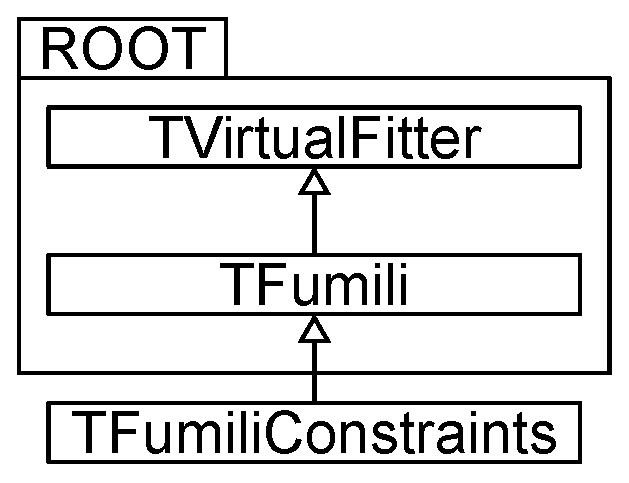
\includegraphics[width=0.4\textwidth]{pics/arch1.eps}

% \begin{figure}[htbp]
% \centering
% \centering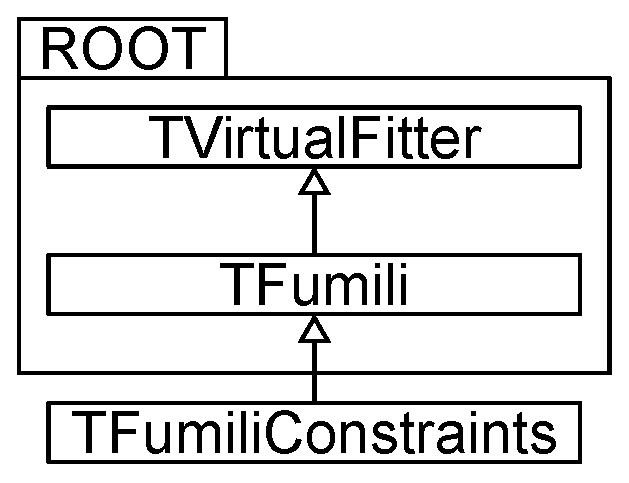
\includegraphics[width=0.35\textwidth]{pics/arch1.eps}
% \caption{
% Схема отношений классов при фитировании.
% Разработанный авторами класс TFumiliConstraints наследует от класса TFumili.
% }
% \label{arch}
% \end{figure}

%фактический user API. Несколько избыточен для статьи и вообще недоработан
% \begin{verbatim}
% void FCN(int & n_par, double * grad,
%          double & val, double * par, int flag);
% /* ... */
% TFumiliConstraints * fum = new TFumiliConstraints;
% // set parameters
% fum->SetParNumber(2);
% fum->SetParameter(0, "#alpha", .5, 0.01, 0, 0);
% fum->SetParameter(1, "#beta", .0, 0.01, 0, 0);
% // set constraints
% fum->SetConstrNumber(1);
% fum->SetConstraint(0, [](double * p){
%   return p[0]*p[0] + .5*p[1] - 1.3;
% });
% fum->SetConstrDeriv(0, 0, [](double * p){ return 2*p[0]; });
% fum->SetConstrDeriv(0, 1, .5);
% // set objective function
% fum->SetFCN(FCN);
% // minimize
% fum->Minimize();
%
% \end{verbatim}


\section{Example: Monte-Carlo simulation}
% \begin{frame}\frametitle{Testing on a ``toy'' sample}
% { \small
A set of 500\,000 $(a,b)$ events, Monte-Carlo generated according to the function
\(1 + x_1a + x_2a^2 + x_3b + x_4b^2\)
with parameters
\{$x_1 = 0.5$, $x_2 = 0.3$, $x_3 = 0.8$, $x_4 = 0.1$\};
and fitted using an event-by-event log.\ likelihood method with constraints
\(x_1^2 + x_1x_4 - x_4^2 = 0.29\), \(x_2^2/x_3 = 0.1125\).
% }

% Results:
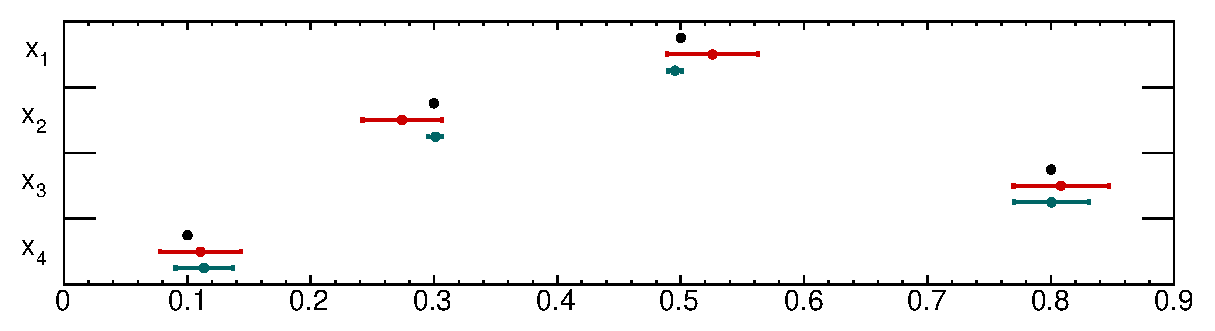
\includegraphics[width=1\textwidth]{pics/drawToy.eps}

\begin{tabular*}{1\textwidth}{@{\extracolsep{\fill}}cccc}\hline\hline
Parameter & True values & Unconstrained fit & Constrained fit \\\hline
$x_1$ & $0.5$ & $0.526 \pm 0.037$ & $0.496 \pm 0.006$ \\
$x_2$ & $0.3$ & $0.274 \pm 0.032$ & $0.301 \pm 0.006$ \\
$x_3$ & $0.8$ & $0.808 \pm 0.039$ & $0.801 \pm 0.030$ \\
$x_4$ & $0.1$ & $0.111 \pm 0.033$ & $0.114 \pm 0.023$ \\\hline\hline
\end{tabular*}

\section{Kinematic fitting at ANKE}
% Kinematic fitting at ANKE
Разработанное расширение было использовано авторами для кинематического фита в реакции $pp \to pp$ на данных, полученных на спектрометре ANKE (Jülich, Germany) [TODO: вставить ссылку на ANKE].

На рисунке \eqref{anke_scheme} можно видеть, что в процессе прохождения протонного пучка через установку часть протонов может отклоняться от направления основного пучка и не фиксироваться установкой, таким образом при анализе данных эксперимента мы можем столкнуться с разницей зафиксированных энергий и количества вещества, вступившего в реакцию с данными, полученными на выходе. Восстановить долю таких ``потерянных'' протонов мы можем, используя инвариант Лоренца $\left|\boldsymbol{P}^{(4)}_\mathrm{beam}+\boldsymbol{P}^{(4)}_\mathrm{targ}-\boldsymbol{P}^{(4)}_p\right|^2 = m_p^2$.

TODO: Добавить, причем тут Polar CMS coordinates.

\begin{figure}[h]
\centering
\centering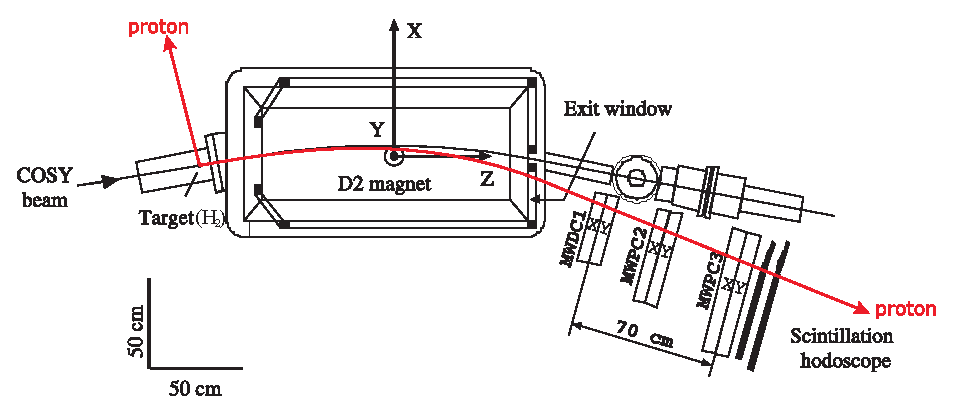
\includegraphics[width=0.8\textwidth]{pics/setup_.eps}
\caption{
Схема прохождения протонного пучка через установку ANKE.
}
\label{anke_scheme}
\end{figure}

% \centering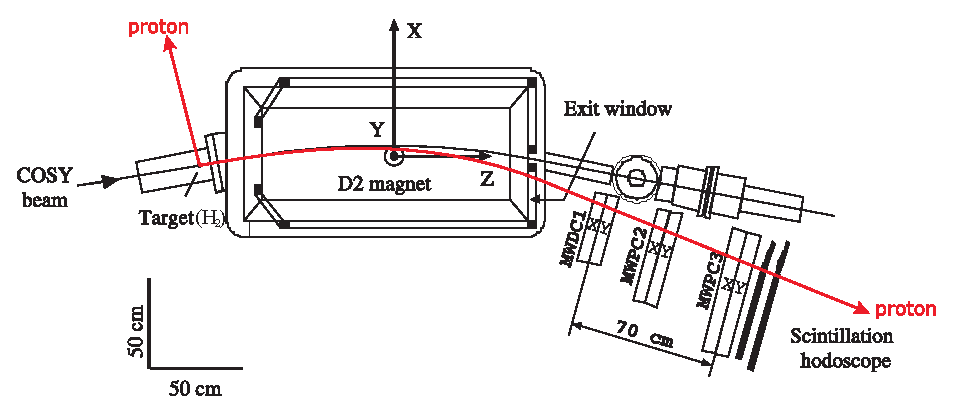
\includegraphics[width=0.8\textwidth]{pics/setup_.eps}

% \large
% \phantom{0}
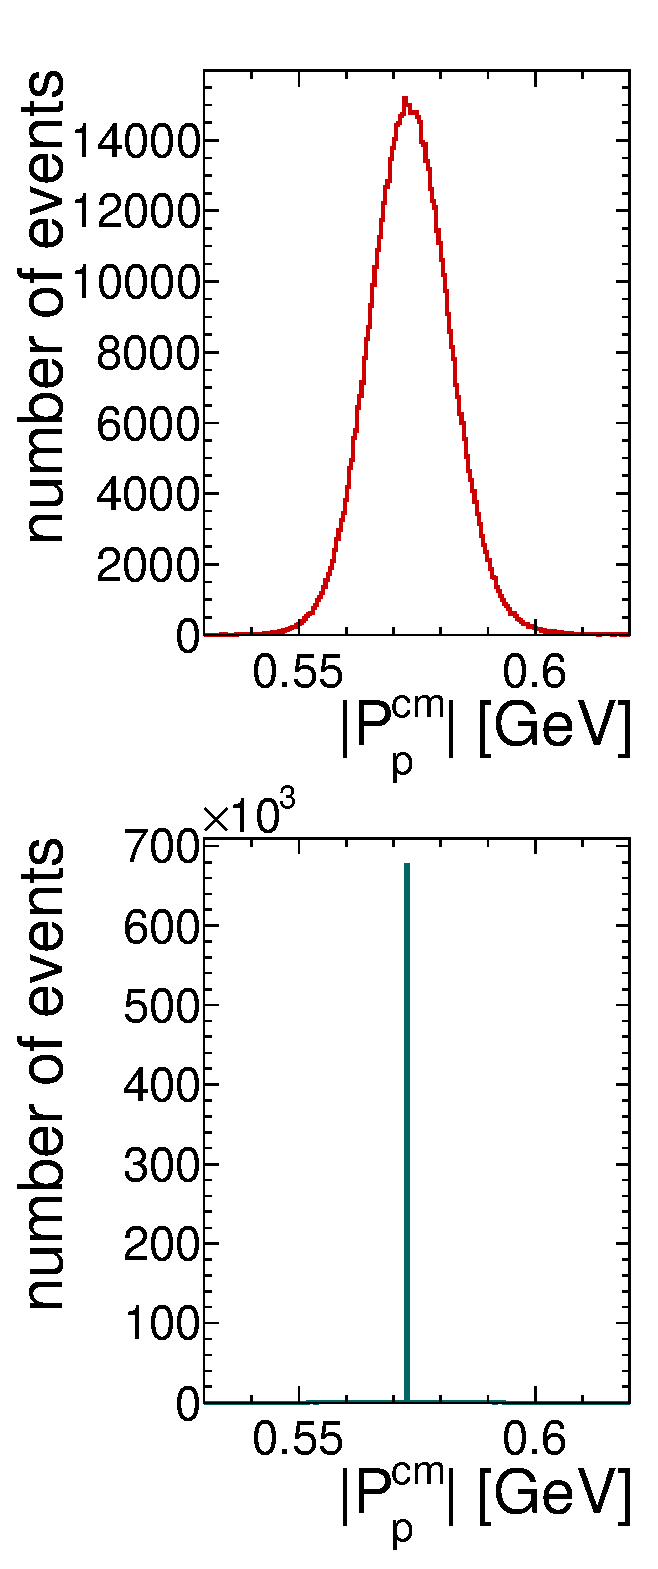
\includegraphics[height=0.7\textheight]{pics/drawMom.eps}
\hfill
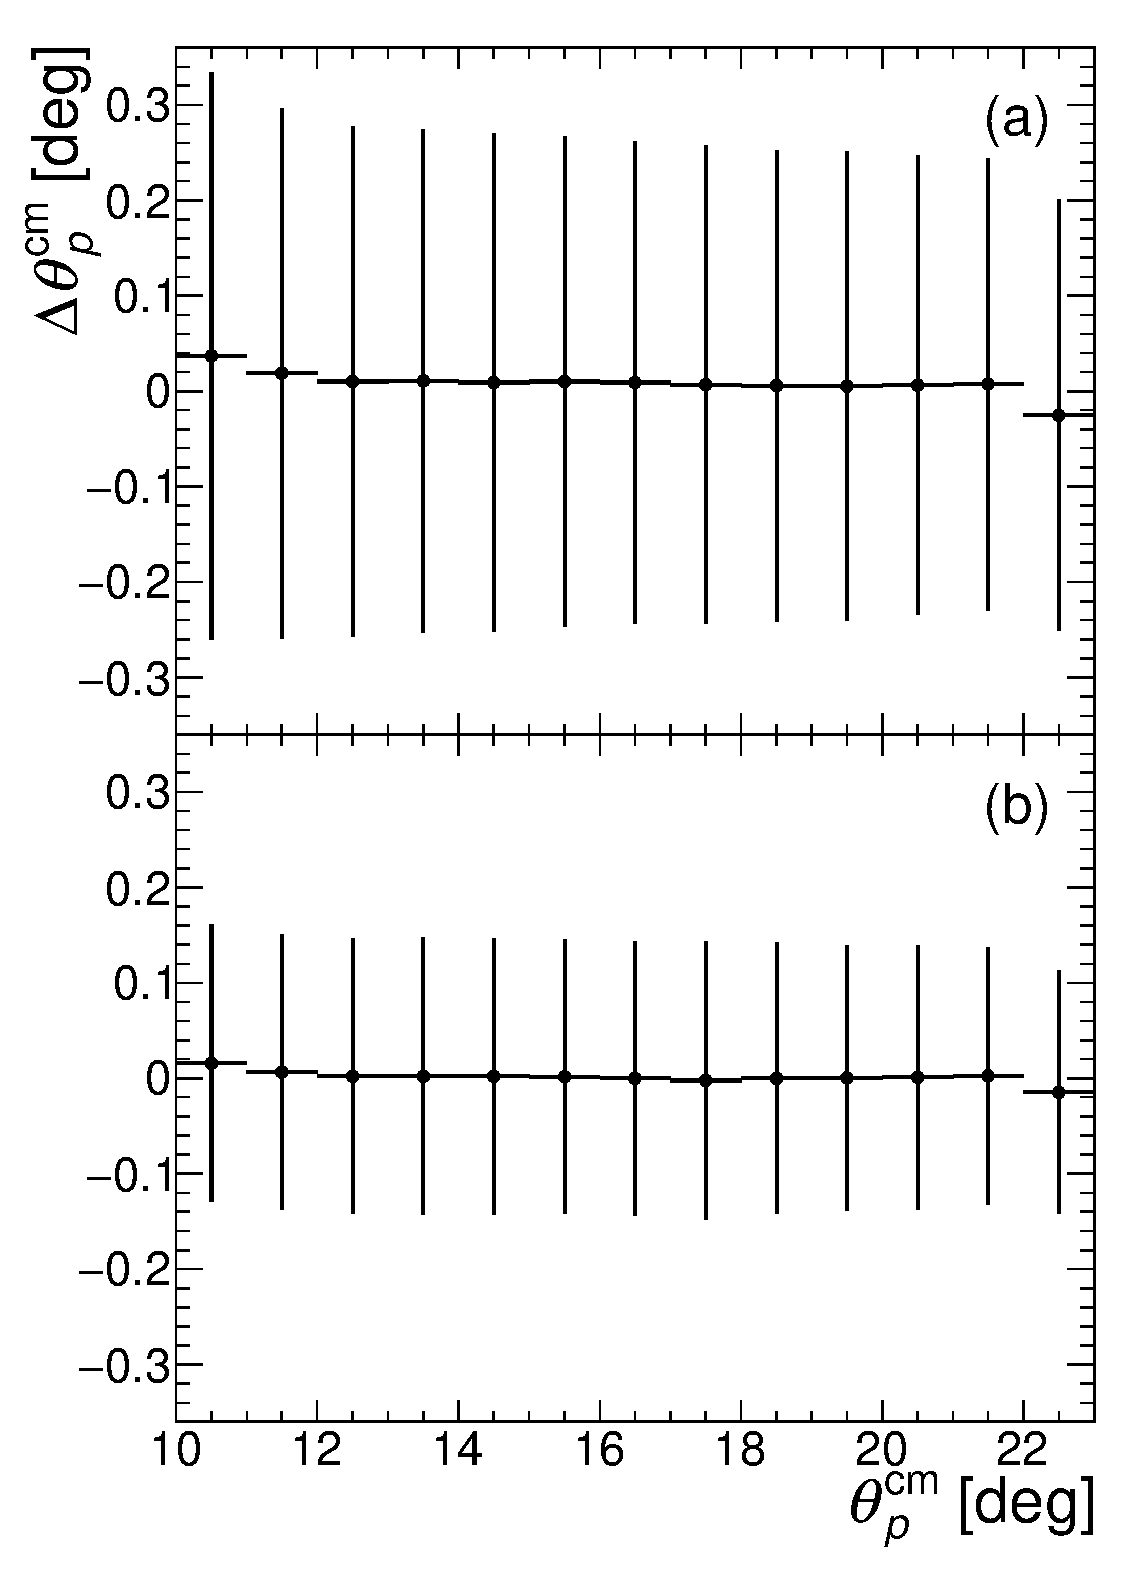
\includegraphics[height=0.7\textheight]{pics/drawTh.eps}
\hfill
% \hspace{1em}
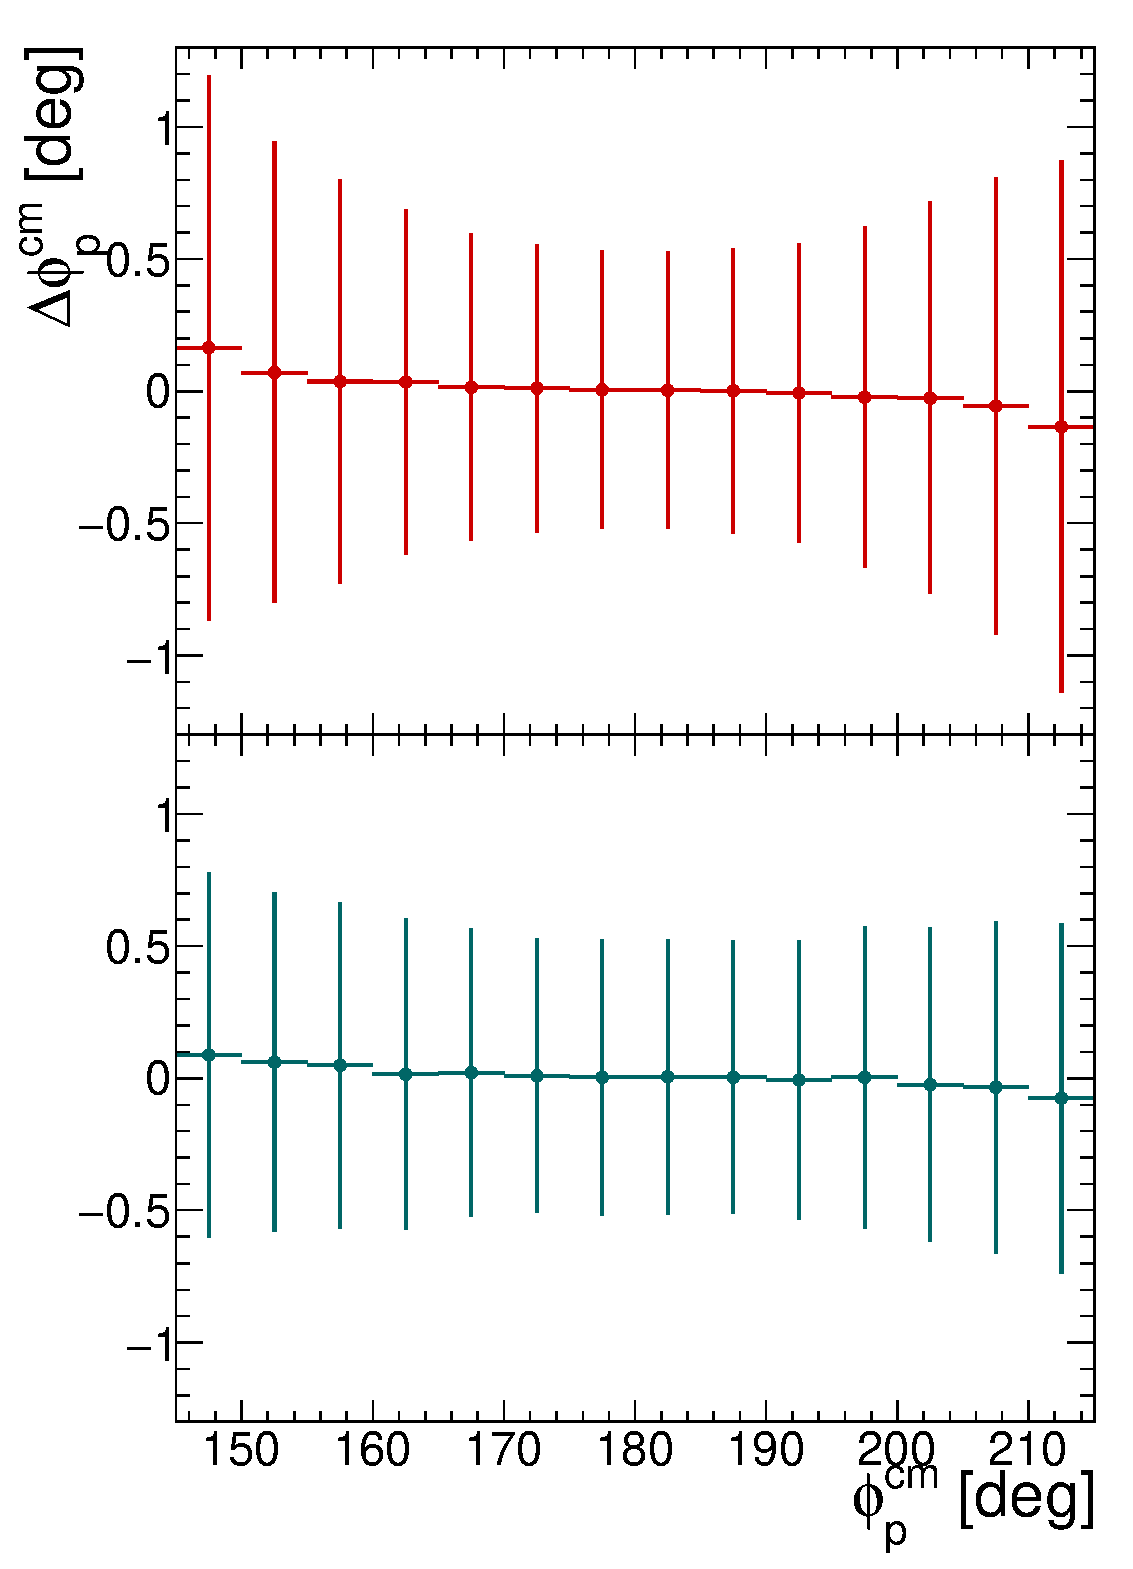
\includegraphics[height=0.7\textheight]{pics/drawPhi.eps}
% \hfill
% \phantom{0}

Errors of reconstructed proton momentum in polar coordinates $(|P_p^\mathrm{cm}|, \theta_p^\mathrm{cm}, \phi_p^\mathrm{cm})$ for the $pp \to pp$ reaction at ANKE, simulated for $T_\mathrm{beam} = 700$~MeV with and without kinematic fitting.

\section{Conclusion and outlook}
% Outlook
\begin{itemize}
\item Improving readability of the code and covering it with tests;
\item Adding the method of Lagrange multipliers to the code;
\item Adding the penalty-function method to the code;
\item Open-source release.
\end{itemize}


\begin{thebibliography}{00}
\bibitem{b1} J.P.~Berge, F.T.~Solmitz, H.D.~Taft, Rev.\ Sci.\ Instr.\ \textbf{32} 538 (1961).
\bibitem{b2} R. Bock, Application of a generalized method of least squares for kinematical analysis of tracks in bubble chambers,       Geneva : CERN, 1960. - 11 p. CERN 60-30 (1960).
\bibitem{b3} G.A. Korn, T.M. Korn, Mathematical handbook for scientists and engineers, McGraw-Hill (1968) 333--335; \foreignlanguage{russian}{Г. Корн, Т. Корн, Справочник по математике для научных работников и инженеров, Наука (1974) 334--336}
\bibitem{b4} P. Avery, KWFIT package\\ URL: \texttt{http://www.phys.ufl.edu/\textasciitilde{}avery/kwfit/}
\bibitem{b5} V.I. Moroz, JINR communications R-1958 (1965)\\ URL: \texttt{http://nu73-73.jinr.ru/\textasciitilde{}cyrkov/MorozJINRCommR1958.pdf}
% \texttt{https://drive.google.com/file/d/1z1hPsccoyXYGA-DT6-7xmeKnYBwPJCS8}
\bibitem{b6} V.S. Kurbatov, I.N. Silin, Nucl. Instrum. Meth. Phys. Res. A 345 (1994) 346--350
% \bibitem{b7} S.N. Dymov et al., Nucl. Instrum. Meth. Phys. Res. A 440 (2000) 431--437
\bibitem{b8} S. Barsov et al., Nucl. Instrum. Meth. Phys. Res. A 462 (2001) 364
\bibitem{b9} V. Komarov et al., Phys. Rev. C 93 (2016) 065206
\bibitem{b10} S. Dymov et al., FdModule framework\\ URL: \texttt{http://nu73-73.jinr.ru/\textasciitilde{}dymov/FdModule/index.html}

\bibitem{anke} ANKE collaboration official web-page\\ URL: \texttt{http://collaborations.fz-juelich.de/ikp/anke/index.shtml} 

% % Zainon, R., Butler, A. P. H., Cook, N. J., Butzer, J. S., Schleich, N., de Ruiter, N., Tlustos, L., Clark, M. J., Heinz, R. & Butler, P. H. (2010). Construction and operation of the MARS-CT scanner,
% % Internetworking Indonesia Journal 2(1): 3–10.
% \bibitem{mars}
% R.~Zainon, A.P.H.~Butler \textit{et al.}, Internetworking Indonesia Journal \textbf{2(1)}, 3--10 (2010).
%
% \bibitem{dicom}
% DICOM standard official site, available at http://dicom.nema.org/standard.html.
%
% \bibitem{turbel}
% H.~Turbell, \textit{Cone-beam reconstruction using filtered back-projection}, Link\"oping University Electronic Press, 189 (2001).
% %
% % and use \bibitem to create references.
% \bibitem{trends}
% I.~Scholl, T.~Aach, T.M.~Deserno \textit{et al.}, Comput.\ Sci.\ Res.\ Dev.\ \textbf{26}, 5--13 (2011).
%
% \bibitem{Roobot}
% C.A.~Roobottom, G.~Mitchell, G.~Morgan-Hughes, Clin.\ Radiol.\ \textbf{65 (11)}, 859--67 (2010).
%
% \bibitem{popularCT}
% T.~Hiroyasu, Y.~Minamitani, M.~Yoshimi, M.~Miki, WORLDCOMP'11 \textbf{2011-MRS-84 (5)} (2011).
%
% \bibitem{hierarhCT}
% S.~Xiao, Y.~Bresler, D.C.~Munson, Proceedings 2003 International Conference on Image Processing \textbf{2}, II–819–22 (2003).
%
% \bibitem{77}
% L.~Feldkamp, L.~Davis, J.~Kress, Journal of the Optical Society of America A \textbf{1(6)}, 612--619 (1984).
%
% \bibitem{bigObserve}
% A.~Belle, BioMed Research International \textbf{2015}, 16 (2015).
%
% % \bibitem{Scherl}
% % H.~Scherl, \textit{Evaluation of State-of-the-Art Hardware Architectures for Fast Cone-Beam CT Reconstruction} (Springer Fachmedien Wiesbaden GmbH, Wiesbaden, 2011) XX, 138
% %
% % \bibitem{Yu}
% % L.~Zhou, J.~Chang, Medical Physics \textbf{39} 4000 (2012)
% %
% % \bibitem{Ramani}
% % S.~Ramani, J.A.~Fessler, IEEE Transactions on Medical Imaging, \textbf{31 (3)}, 677 (2012)
% %
% % \bibitem{Yan}
% % G.~Yan, S.~Zhu, Y.~Dai, C.~Qin, Journal of X-Ray Science and Technology \textbf{16 (626)} 225--234 (2008).
%
% \bibitem{76}
% B.~Meng, G.~Pratx, L.~Xing, Med.\ Phys.\ \textbf{38(12)} 6603--6609 (2011).
%
% % \bibitem{77}
% % C.F.~Mackenzie, P.~Hu, A.~Sen et al., AMIA Annual Symposium Proceedings \textbf{2008} 318--322 (2008)
%
% \bibitem{chinese}
% C.-T.~Yang, C.-T.~Kuo, W.-H.~Hsu, W.-C. Shih, Proceedings of the 7th international conference on Advances in Grid and Pervasive Computing \textbf{7296}, 338--349 (2012).
%
% \bibitem{HDFS} HDFS documentation, available at http://hadoop.apache.org/docs/current/hadoop-project-dist/hadoop-hdfs/HdfsDesign.html.


%###################################################################################
% \bibitem{RefJ}
% Format for Journal Reference
% Journal Author, Journal \textbf{Volume}, page numbers (year)
% Format for books
% \bibitem{RefB}
% Book Author, \textit{Book title} (Publisher, place, year) page numbers
% etc
\end{thebibliography}
\end{document}
